\section{Introduction} \label{sec:intro}
% Introduction
In 2017, the European Union counted around $25300$ fatalities on the EU roads, of which 46\% were \glsfirst{VRU} (e.g. pedestrians and (motor-)cyclists). Although the EU roads account for the safest roads in the world, the number of road fatalities have stagnated in the past few years. At this rate, the EU's goal of reaching fewer than $16000$ fatalities in 2020 could not be achieved. Especially vulnerable road user fatalities have not decreased at the same pace as the overall population. Any progress to increase the safety of \gls{VRU} will have a significant impact to the road fatality rate. \cite{vademecumeu2018road} \\

\glspl{AV} are expected to increase road safety, since more than 90\% of the accidents is caused by human error \cite{eu2020website}, and autonomy would erase the effects of human error \cite{cui2019review}. However, \glspl{AV} are not yet safe enough to deploy on the roads and still a lot of research should be done before fully autonomous vehicles can be introduced to the market \cite{okuda2014survey} \cite{cui2019review}. \\

One of the current challenges to autonomous driving is to capture road user intent and to make accurate real-time trajectory predictions of other road users \cite{ohn2016looking}. Especially predicting the behavior of \glspl{VRU} is important \cite{ohn2016looking} \cite{cara2015classification} because good anticipation of a \gls{VRU}'s behaviour results in faster reactions and thus can prevent more accidents \cite{djuric2020uncertainty}. Predicting \gls{VRU} behavior is additionally challenging compared to predicting other (motorized) road users, because the motion patterns of \glspl{VRU} are complex and mutable depending on the static and dynamic obstacles they encounter \cite{chou2020predicting}. Therefore, a motion prediction method is needed that can also accurately predict the motion of \glspl{VRU}.\\

%TODO: New paragraphs
Current trends in research on motion prediction methods show two frequently used methods: object-centered motion prediction and \glsfirst{OGM} prediction. The first uses prior state and semantic information of annotated objects (from object detections) in the \gls{AV}'s environment to perform motion predictions in the form of state estimations. The second makes use of an \glsfirst{OGM} to capture the \gls{AV}'s environmental context and predict future \glspl{OGM} based on that context. An \gls{OGM} is a top-down representation of the environment in the form of a small grid. Each cell in the grid specifies whether it is empty, occupied, or unknown corresponding to the \gls{AV} sensor's perception of the environment. An example of an \gls{OGM} is shown in figure \ref{fig:ogm_example}. Both methods have their advantages and disadvantages to use for motion prediction. \\

\begin{figure}[h]
	\centering
	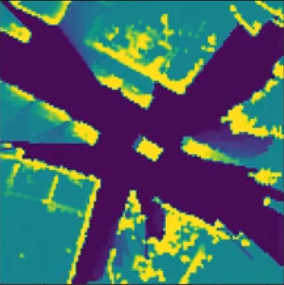
\includegraphics[width=0.3\linewidth]{Figures/Title_Page_OGM}
	\caption{An example of an \glsfirst{OGM}. Blue: Emtpy, Yellow: Occupied, Green: Unknown. The ego-vehicle (from which the sensor data is recorded) is represented by the yellow rectangle (occupied area) at the center of the \gls{OGM}.}
	\label{fig:ogm_example}
\end{figure}

%%%%%%%%%%%%%
%% Miscellaneous
% \gls{OGM} prediction does not require semantically labeled ground truth data \cite{dequaire2018deep} unlike the object centered approach.  
% WHY OGM as OUTPUT is GOOD? Because it can be used immediately for path planning..
%%%%%%%%


% object prior information using object detection vs raw data use
\cite{hormann2020long} describes the need to use object hypotheses (from object detection methods) in prediction methods. Object-centered prediction methods detect and label objects to link prior dynamic information to them (e.g. velocity and orientation) which is used to compute the predictions. On the other hand, \glspl{OGM} do not directly incorporate the dynamics of the objects within it \cite{itkina2019dynamic}. Without the use of object detection and labeling, \glspl{OGM} exclude object category information from each grid cell. This makes it challenging for \glspl{OGM} prediction methods to extract dependencies between the independent grid cells and to consider dynamic constraints of category-specific traffic actors. \cite{wu2020motionnet} \cite{hormann2020long}. The inability of \gls{OGM} prediction methods to recognize objects and their shapes through grid cell dependencies might cause objects to be removed from or blurred in the predictions \cite{lange2020attention}. An example of blurring in \gls{OGM} predictions is shown in figure \ref{fig:ogm_blurr}. \\

\begin{figure}[h]
	\centering
	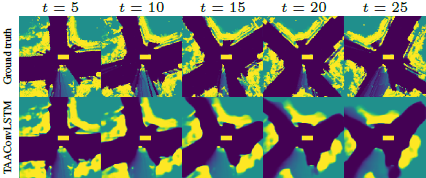
\includegraphics[width=0.5\linewidth]{Figures/Introduction/Blurring_OGM}
	\caption{An example of blurring of an object in the \gls{OGM} predictions\cite{lange2020attention}. Blue: Emtpy, Yellow: Occupied, Green: Unknown. The object below the yellow rectangular center vehicle loses its shape and certainty and ends in an uncertainty blurr as time progresses.}
	\label{fig:ogm_blurr}
\end{figure}

The downside, however, of object-centered prediction methods is that errors in the object detection phase are often impossible to recover due to a loss of information \cite{li2020end}. The object detection methods might remove uncertain detections or fail to detect objects, which are consequently not considered in the predictions. Furthermore, object-centered methods can be limited in their generalization abilities because they consider only certain detected contexts resulting from the object extraction from the raw sensor data \cite{itkina2019dynamic}. \\

As an advantage, \gls{OGM} prediction methods are generated directly from raw sensor data. A variety of sources for raw sensor data can be fused to generate an \gls{OGM} making it independent from a sensor's specifications \cite{hoermann2018dynamic}. This provides more occupancy information of the environment compared to object-centered approaches. Moreover, in \gls{OGM} predictions, all grid cells are considered, so no information is lost due to object detection errors \cite{wu2020motionnet}. Another benefit from directly using raw sensor data to generate \glspl{OGM} is that \gls{OGM} generation methods can directly incorporate probabilistic occupancy estimates which can benefit uncertainty predictions \cite{hoermann2018dynamic}. \\

%% processing spatial relations and interactions 
Furthermore, a challenge for object-centered prediction is to predict the future trajectories for all objects in the scene. This often requires additional computations for every actor (of which an example is shown in figure \ref{fig:obj_comp}), or interaction in the scene, which can be problematic to scale for dense urban environments \cite{meyer2020laserflow} \cite{zhao2019multi} \cite{ettinger2021large}. By contrast, an \gls{OGM} does not require more computations for additional actors in its environment. An \gls{OGM} captures spatial context information because the relative distances of the measurements within the recorded environment correspond to the relative distances between the \gls{OGM}'s grid cells \cite{hoermann2018dynamic}. Since \glspl{OGM} have an image-like data structure, \glspl{CNN} and other image-based deep learning techniques can be used to extract contextual information from the grid cells \cite{hoermann2018dynamic} \cite{itkina2019dynamic}.  \\

\begin{figure}[h]
	\centering
	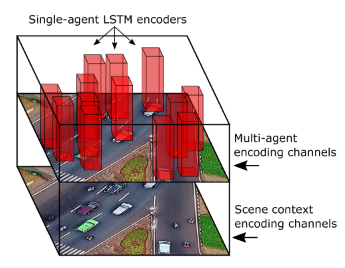
\includegraphics[width=0.4\linewidth]{Figures/Introduction/Multi-agent_obj_cent}
	\caption{An example of multi-object prediction in object-centered prediction methods \cite{zhao2019multi}. For every detected object in the scene, an additional computation is done (in the form of an LSTM encoder and decoder).}
	\label{fig:obj_comp}
\end{figure}

Since both prediction methods have their advantages and disadvantages, both are worth investigating. In this literature study, the choice is made to focus on \gls{OGM} prediction methods. This literature study gives an overview of what the current research areas and challenges for the future are regarding motion prediction using \glspl{OGM}. The conclusion of this study forms the basis for the Master thesis research proposal at the end of this literature review. \\

In the following sections of this introduction, first, the problem of motion prediction is described. Then, current solutions to motion prediction challenges and their limitations are briefly discussed. After discussing the challenges and limitations of current solutions, it is explained why \gls{OGM} prediction methods are a promising all-encompassing solution to those current challenges. Then, one main research question and four sub-questions are posed to investigate the stated motion prediction problem regarding \gls{OGM} prediction methods. The following chapters provide information from literature to answer the main and sub-questions posed in this introduction. This chapter ends with a short overview of the content of each chapter.

\subsection{Problem Description} 
%Problem
The problem of motion prediction is an inferencing task. Based on evidence in the form of current and/or past observations and experiences, future states (trajectories) of one or more actors (i.e. traffic participants such as cars and \glspl{VRU}) must be predicted for a pre-determined time horizon, within a certain accuracy and certainty, which needs to be executed within a specific time limit. This problem statement will be explained more elaborately in these following paragraphs. \\

The evidence that supports the actor's predictions can have the form of current and/or past observations, and experience. The current and past observations are sensor data acquired from the environment (observations) by either static observers (the sensors are static and record the environment) or dynamic observers (the sensors move within the environment while recording it) or both.
Then, experience is the generalization of traffic in patterns, including traffic behavior and traffic environments. These generalizations can be based on statistics, they can be based on assumptions, and they can be learned using historic observations. \\

Based on the investigated literature, the predicted future states can be represented as either of the following forms. The first form is object centered prediction, while the second form is based on \gls{OGM} prediction. 

\begin{enumerate}
	\item The predictions are estimated future state values of an actor's centroid, including its coordinates and sometimes orientations, which are projected into the environment representation (Figure \ref{fig:pred_froms} a and b). \cite{cui2019multimodal} \cite{djuric2020uncertainty} \cite{rhinehart2019precog} \cite{kawasaki2021multimodal} \cite{li2020end} \cite{luo2018fast}
	\item The predictions are estimations of the entire future environment representation (Figure \ref{fig:pred_froms} c). \cite{itkina2019dynamic} \cite{lange2020attention} \cite{toyungyernsub2020double} \cite{mohajerin2019multi} \cite{dequaire2018deep} \cite{wu2020motionnet} \cite{hoermann2018dynamic} \cite{schreiber2019long}
\end{enumerate}

\begin{figure}[h!]
	\centering
	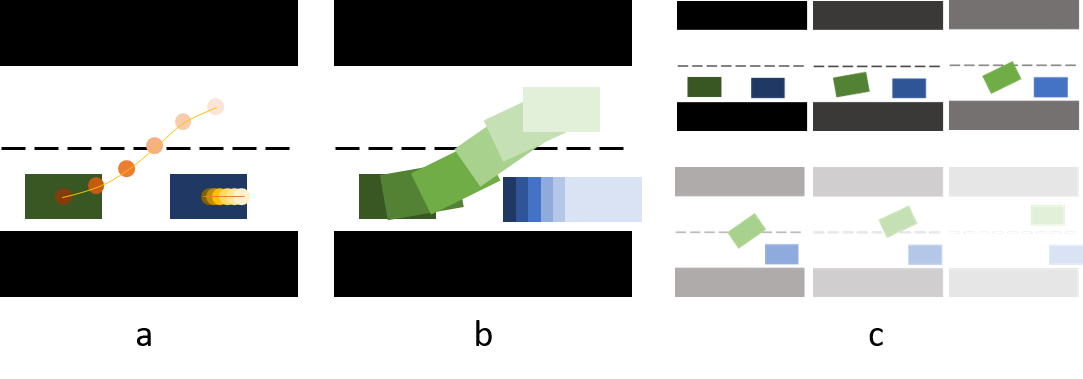
\includegraphics[width=0.8\linewidth]{Figures/Introduction/Prediction_forms}
	\caption{The prediction forms encountered in the literature. The black and white parts represent a road. The green and blue squares are representations of vehicles. The predictions are shown using a more fading color the further the prediction goes into the future. Figure a shows the prediction of future centroids projected into the environment representation. Figure b shows the prediction of future actor representations within the environment (the complete vehicles are predicted instead of the centroids only). Figure c shows the prediction of the entire future environment. In this case, also a prediction of the environment (road) is provided.}  
	\label{fig:pred_froms}
\end{figure}

Finally, the problem statement mentions a time horizon, that the predictions must be within a certain accuracy and certainty, and that it needs to be executed within a specific time limit. The time horizon is the amount of time into the future that the prediction must span. Ideally, the time horizon, the accuracy, the certainty, and the execution time of the predictions should be infinitely, exact, complete, and instantaneous, respectively. However, this is not possible in practice. Therefore, I think a suitable prediction method should predict further into the future, be more accurate, have more certainty, and be faster than a human could perform the task. Within the context of \glspl{AV}, this is a reasonable requirement in order for the \gls{AV} to be able to perform safer than humans can.   


\subsection{Current Solutions}
Over the past decade, much research has been done to find methods that solve the previously mentioned motion prediction problem. Table \ref{tab:overview_mot_pred} in Appendix \ref{app:appendixA} shows an overview of recent motion prediction papers and their respective methods. It is notable that most methods use a form of deep learning to predict trajectories in any of the forms as described in the problem description. What is also striking, is that relatively few papers have performed research which includes \glspl{VRU} in which the observer is dynamic (from a vehicle's point of view). Still, it is important that \gls{VRU} behavior prediction is investigated. Collisions with \glspl{VRU} are likely to be fatal which makes accurate and early motion prediction necessary in order to respond safely to their actions \cite{rehder2018pedestrian}, \cite{chou2020predicting}, \cite{uah2020d4}. Therefore, \gls{VRU} behavior prediction is a relevant research topic regarding \glspl{AV}.\\
A major challenge in this research area is to predict \gls{VRU} motion for the long term. However, research on this topic faces a multitude of challenges. Accurate long-term predictions require the incorporation of environmental and social context. Moreover, implementing uncertainty and multimodality of the predictions and making the predictions fast enough for real-time applications in \glspl{AV} are also challenges that need to be solved. These major challenges and recent research to find solutions are described in the following subsections. 

\subsubsection{Long-term motion prediction}
For motion prediction, a prediction for which the prediction time horizon is more than 2 seconds is considered long-term \cite{hormann2020long}. Compared to other road users, \glspl{VRU} are highly maneuverable which makes it challenging to predict their behavior, especially for the long-term \cite{xiong2019recurrent}, \cite{rehder2018pedestrian}, \cite{rehder2018pedestrian}. Most prediction models assume that \gls{VRU} behavior is intention-driven and that those intentions can be inferred from certain cues, other than dynamics \cite{rehder2018pedestrian}. Therefore, detecting cues related to \gls{VRU} behavioral changes is important for achieving accurate long-term predictions \cite{pool2017using}. These cues can be related to the \gls{VRU}'s environment (e.g. traffic lights, zebra's, obstacles) or to the \gls{VRU}'s social interactions (e.g. evasion of other \gls{VRU}'s, distancing due to social norms, nearing another \gls{VRU}). The following two paragraphs elaborate on the incorporation of environmental and, respectively, social context in prediction models. Besides using cues to predict \gls{VRU}'s behavior, implementing the uncertainty of the predictions and incorporating multimodality is also researched, as well as making the models fast enough so that they can be implemented real-time on \glspl{AV}. These topics are also discussed below. 

\subsubsection{Environmental context}

Environmental context consists of the static and dynamic obstacles and semantic meaning within an actor's surroundings. Research suggested to incorporate environmental context because an actor's trajectory is highly influenced by its environment, since scene context can constrain the actor in its planned motions \cite{chou2020predicting} \cite{pfeiffer2018data} \cite{sadeghian2019sophie} \cite{manh2018scene}. Especially to anticipate critical situations, taking into account the environmental context is expected to increase the prediction accuracy \cite{uah2020d4}. An example of how the use of traffic light information influences the predictions is shown in figure \ref{fig:env_cont}. The challenge is how to model that environmental context so that it is semantically representative, highly discriminative and generalizable to a variety of complex scenes. This way, it can be used as evidence to enable inferences about an actor's future trajectory \cite{varshneya2017human}. \cite{pool2017using} shows that leveraging prior knowledge about an actor's environment can improve the trajectory predictions. Therefore, they suggest to extend the incorporation of environmental context even more with the expectation that it will further increase the prediction accuracy.  

\begin{figure}[h!]
	\centering
	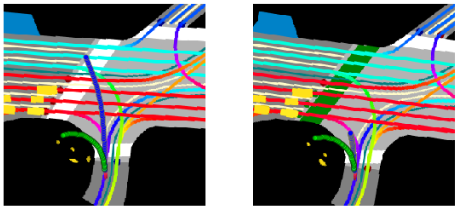
\includegraphics[width=0.5\linewidth]{Figures/Introduction/Environmental_Context_TRaffic_Light_Chou}
	\caption{An example of how the environmental context can be used to influence the predictions. On the left, the prediction (the blue trajectory) of the bicyclist (red) is shown when the traffic light in the scene is green. On the right, the bicyclist's prediction is shown when the traffic light turned red. The green trajectory is the ground truth. \cite{chou2020predicting}}  
	\label{fig:env_cont}
\end{figure}


\subsubsection{Social Context}
Social context consists of the static and dynamic actors, their semantic meaning, and their interactions within an actor's surroundings. When an actor navigates, it constantly tries to anticipate movements of surrounding actors to envision more than one feasible path it could take in order to adjust its own path and maneuver past or aside those surrounding actors \cite{sadeghian2019sophie}, \cite{manh2018scene}. Figure \ref{fig:soc_cont} shows how \cite{sadeghian2019sophie}'s prediction method takes into account social context. Therefore, one of the main factors that influence an actor's behavior is the its social context. It is expected that by incorporating social context into prediction models, the accuracy will increase significantly \cite{pfeiffer2018data}. 
Especially for pedestrian behavior, the social and environmental context is expected to be the leading evidence for predicting their behavior because pedestrians \airquote{are not expected to use any active forms of communication when interacting with vehicles and other road users} \cite{uah2020d4}. 

\begin{figure}[h!]
	\centering
	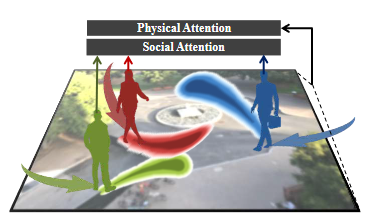
\includegraphics[width=0.4\linewidth]{Figures/Introduction/Social_context_Sadeghian}
	\caption{A schematic of how \cite{sadeghian2019sophie} uses the social context, and the scene context, to predict the behavior of the pedestrians (the green, red, and blue surfaces). The pedestrians are predicted to avoid each other while continuing in the general direction they walked in the past (the arrows). \cite{sadeghian2019sophie}'s method predicts physically and socially plausible trajectories.}  
	\label{fig:soc_cont}
\end{figure}

\subsubsection{Uncertainty and Multi-modality}
For the safety of AVs, uncertainty estimations for predictions are critical \cite{djuric2020uncertainty}. If an AV is aware of the confidence of its predictions, it can adjust its planned course to minimize the risk of collisions \cite{huang2019uncertainty}. For example, if an AV predicts that a pedestrian will not cross the road, but the confidence of that prediction is very low, the AV can adjust its course by leaving more room for the pedestrian in case the prediction is false. Without knowing the confidence of a prediction, such risk-avoiding course adjustments cannot be made. Besides including uncertainty estimations, it is important that predictions are multimodal. VRU behaviour is inherently multimodal because they easily change their course which is highly dependent on their environment \cite{cui2019multimodal}, \cite{tang2019multiple}. Incorporating multimodality is a challenge, because it requires good probability estimations and knowledge of the different modes. It either requires explicit labeling of the modes prior to training \cite{tang2019multiple}, or the modes could be learned. Because probability estimations are needed to make multimodal predictions, these methods are often researched together. \\

\cite{keller2013will} compares four different multimodal prediction models related to Bayesian principles. These models return the probability of stopping (whether a nearing pedestrian will stop, instead of cross the road). However, only two motion modes are considered in this research. \cite{pool2017using} Uses a Mixture of Linear Dynamical Systems to predict the probabilities of a cyclists going in one of the five pre-determined direction modes. This model also takes into account information about the road topology to enhance the predictions. The downside of these Bayesian models is that the computation time increases when more modes are added and when more context information is incorporated in the predictions. Moreover, adding more modes is a challenges in complex environments in which it is unclear what directions an actor can go to. Therefore, deep learning models are devised that can include multimodality in the predictions by learning the modes in a latent space and incorporating learned features of the VRU's context. \\
\cite{rehder2018pedestrian}, \cite{cui2019multimodal}, \cite{brito2020social} investigated deep learning models that, respectively, predict multimodal trajectories by training a network to learn the parameters of a Mixture Density Network that predicts multiple trajectories, train a network to choose the best of M hypothetical trajectory modes, and train a variational RNN that learns a conditional distribution of available modes from which the output Gaussian Mixture Model can be sampled. Although these methods all provide probabilities for the different available trajectory modes, still they do not provide a confidence estimation the model has about the multimodal predictions. \cite{huang2019uncertainty}'s research adds a confidence estimator to their multimodal prediction method that estimates the confidence of multiple predictors (See figure \ref{fig:multimod}). The predictor with the highest confidence value is considered for the trajectory prediction. 

\begin{figure}[h!]
	\centering
	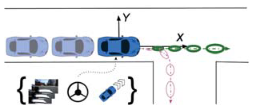
\includegraphics[width=0.4\linewidth]{Figures/Introduction/Multimodality_Huang}
	\caption{A schematic of how multimodal predictions can be made, given a past trajectory. Since the road allows for two directions the vehicle can move in, two predictions are made. One prediction in green, going straight. The other in red, going to the right. The prediction that goes straight forward is given the highest confidence value (thick green), which means that that trajectory is considered for the prediction.  \cite{huang2019uncertainty}}  
	\label{fig:multimod}
\end{figure}

\subsubsection{Real-time motion prediction}
Fast real-time computation is important in order to implement the prediction model on AVs. 
\cite{djuric2020uncertainty} Addresses the importance of real-time execution of prediction models. They state that certain prediction methods (e.g. Bayesian Networks and Inverse Reinforcement Learning) are inefficient and thus not feasible for real-time applications such as AVs. Therefore, it is important that the prediction methods are efficient enough so they can be applied online in AVs to increase VRU safety. Their method of using a CNN to predict future trajectories was succesfully tested real-time in an AV. However, this method only predicts future trajectories of vehicles, not VRUs. \\
\cite{brito2020social} stresses the importance for real-time predictions for applications in AVs as well. They developed the Social-VRNN that takes samples from a variational RNN's conditional distribution to predict pedestrian trajectories. Previous research used other methods, such as Generative Adversarial Networks (GANs), which required more samples for accurate predictions compared to the Social-VRNN, making the Social-VRNN much faster. However, this method does not yet perform in real-time.  \\
\cite{chou2020predicting} aims for the most efficient motion prediction models without it affecting the accuracy because it "is necessary to achieve real-time inference onboard an SDV in crowded urban environments comprising large number of VRUs" \cite{chou2020predicting}. Without real-time online motion prediction, AVs cannot make use of these methods and the safety of VRUs will not improve. They developed a real-time motion prediction method, using a CNN, for all road users. Their solution shows promising results, but the dataset requires more VRU data to match the state-of-the-art prediction accuracy. 

\subsubsection{The promising solution}
The state-of-the-art research in the previous paragraphs show that Deep Learning methods provide means to include environmental and social context, as well as uncertainty information, to make better, long-term, path predictions including those of \glspl{VRU}. Several Deep Learning methods use \glspl{OGM}, a grid-based representation of the environment obtained from sensors on \glspl{AV} (e.g. from a LiDAR, camera, or radar), as input data to predict future \glspl{OGM} for the long-term. \glspl{OGM} contain occupancy data of the \gls{AV}'s environment which is often extended with uncertainty information of the occupied areas. 
Since an \gls{OGM}'s form is similar to an image - a matrix containing values between 0 (Empty) and 1 (Occupied) - convolutional neural networks can be used to efficiently extract useful features from it \cite{albawi2017understanding}. Then, a sequential neural network can be used to process a sequence of the extracted features to capture the past states and behavior of the \gls{AV}'s environment. The information of the past is then used by the neural network to generate \gls{OGM} predictions that describe the future environment of the \gls{AV}. \\
Furthermore, the \gls{OGM} can be extended with additional information layers such as semantics and dynamics of the occupied regions. This literature study expects that predicting \glspl{OGM} is more accurate than predicting in other forms of environment representation. Also for long-term predictions, due to the amount of information that can be stored in the \gls{OGM}. Attempts to make real-time \gls{OGM} predictions are succeeding (Mohajerin \cite{mohajerin2019multi} shows that it can take 60ms to predict \glspl{OGM} 1s into the future), making these methods, using \glspl{OGM} as environment representation, a promising one for motion prediction research. All in all, the motion prediction methods that use \glspl{OGM} can provide solution to all challenges stated in the previous paragraphs. That is why \gls{OGM} prediction is a promising solution that is worth investigating, which leads to the following section about this literature reviews research questions. \\

% TODO: Research questions are adjusted
\subsection{Research Questions}
Because of the potential of \glspl{OGM}, this literature review focuses on the prediction of \glspl{OGM} using Deep Learning. Currently, state-of-the-art research regarding motion prediction in traffic scenes makes use of \glspl{OGM}. To give an overview of these \gls{OGM} prediction methods and to find out which method provides the best predicitons, the following main research question is asked: \textit{"What is a suitable method to perform traffic scene \gls{OGM} prediction using Deep Learning?"} \\

In this review, several sub-questions are asked in order to answer the main question. The reasoning behind the sub-questions is followed by the sub-questions themselves and are described below. \\ 


First, it is important to know what an \gls{OGM} is and how they can be generated from an \gls{AV}'s sensor data. Research shows that \glspl{OGM} can be generated using several methods \cite{collins2007occupancy} \cite{ribo2001comparison} \cite{thrun2003learning}. Besides several generation methods that compute occupancy information for each \gls{OGM}'s grid cell, the \glspl{OGM} can also be extended with other information such as semantics \cite{lu2019monocular}, dynamics \cite{nuss2018random}, and 3D information \cite{degerman20163d}. Combinations of the different generation methods and data extensions will result in different \gls{OGM} forms. This leads to the first sub-question: \textit{What \gls{OGM} form is good to use in \gls{OGM} prediction methods?} \\

Second, to generate the \glspl{OGM}, a dataset should be used that contains sequences of traffic scene sensor data from an \gls{AV}'s point of view. It is important that occupancy information can be extracted from the data. Additionally, it is a perk if the datasets also contains 3D, semantic, or dynamic information about the traffic scenes for the extended \gls{OGM} forms. There exist several datasets (view table \ref{tab:datasets_overview}) that contain this kind of data. To find out which of these datasets is the best to use for \gls{OGM} generation and prediction, the second sub-question is asked: \textit{What is a suitable dataset to generate \gls{OGM} sequences for \gls{OGM} prediction from?} \\

Third, to determine which \gls{OGM} prediction method performs best, the quality of the \gls{OGM} predictions need to be evaluated per method so the different methods can be compared. When evaluating, the \gls{OGM} predictions will be compared to the ground truth \glspl{OGM}. The more the predictions are similar to the ground truth, the better that prediction method performs. Evaluation can be done by visually comparing the predictions to ground truth \glspl{OGM} \cite{ribo2001comparison}. However, this evaluation method is subjective and thus can result in unreliable performance scores. Therefore, \cite{collins2007occupancy} summarizes some quantitative evaluation methods that use image similarity principles to evaluate \glspl{OGM}. Quantitative metrics can provide an objective means for performance evaluation. However, each metric measures a different aspect of the \gls{OGM}. It is therefore important that a metric is chosen that best evaluates the similarity accuracy between \glspl{OGM}. This leads to the third sub-question: \textit{What is a suitable quantitative metric to determine the accuracy of a predicted \gls{OGM}?} \\

Fourth, there are several state-of-the-art deep learning methods that perform \gls{OGM} prediction. To find out which of those methods are the best ones, they must be evaluated and compared with each other. To answer the main questions, this fourth sub-question is asked: \textit{What is a good Deep Learning method to generate \gls{OGM} predictions?}

\subsection{Chapter overview}
The posed research questions will be answered in the following chapters of this literature review. Chapter \ref{sec:ogm} provides information about \glspl{OGM} and answers the first sub-question. In chapter \ref{sec:datasets}, criteria are set which an ideal dataset should meet to use it for \gls{OGM} prediction. This chapter will answer the second sub-question. The third sub-question will be answered in chapter \ref{sec:metrics}, in which several metrics to determine the quality of \glspl{OGM} are compared according to some criteria that are required for accurate and safe (related to \gls{AV}'s) error estimations of \gls{OGM} predictions. The fourth sub-question will be answered in chapter \ref{sec:ogm_methods}, in which an overview of \gls{OGM} prediction methods using deep learning is provided. Chapter \ref{sec:conclusion} contains a conclusion in which the main research question of this literature review is answered. Then, chapter \ref{sec:future} discusses some topics for future work that result from this literature study. The final chapter is a research proposal for my Master thesis to which the conclusion of this literature review provides the basis.



%% After the Challenges: Each challenge becomes a topic/section
%% Long term motion prediction: discuss most used methods up until deep learning methods
%% Discuss how later the incorporation of environment, social, uncertainty/mutlimodality was also incorporated
%% And what methods are used for that
%% Dicuss Why real-time motion prediction is important and what the fastest computation times are for each other challenge
%% And how faster methods can be researched 
%%

%%% NEW LIT PART

%% Before, the main challenges to motion prediction are described. Then, ... thought of using OGMs to predict the future because in an OGM env and social context can be incorporated, multimodal paths and uncertainty can be computed, and some prediction methods can even perform real-time. But what are the advantages and disadvantages? Is it really better?



